\documentclass[
    reds, % Saisir le nom de l'institut rattaché
    il, % Saisir le nom de l'orientation
]{heig-tb}

\usepackage[nooldvoltagedirection,european,americaninductors]{circuitikz}

\signature{mbernasconi.svg} % Remplacer par votre propre signature vectorielle.

\makenomenclature
\makenoidxglossaries
\makeindex

\addbibresource{bibliography.bib}

\usepackage{etoolbox}
\renewcommand\nomgroup[1]{%
  \item[\bfseries
  \ifstrequal{#1}{A}{Constantes physiques}{%
  \ifstrequal{#1}{B}{Groupes}{%
  \ifstrequal{#1}{C}{Autres Symboles}{}}}%
]}

\newcommand{\nomunit}[1]{%
\renewcommand{\nomentryend}{\hspace*{\fill}#1}}

\nomenclature[A, 02]{\(c\)}{\href{https://physics.nist.gov/cgi-bin/cuu/Value?c}
{Vitesse de la lumière dans le vide}
\nomunit{\SI{299792458}{\meter\per\second}}}

\nomenclature[A, 03]{\(h\)}{\href{https://physics.nist.gov/cgi-bin/cuu/Value?h}
{Constante de Planck}
\nomunit{\SI[group-digits=false]{6.62607015e-34}{\joule\per\hertz}}}

\nomenclature[A, 01]{\(G\)}{\href{https://physics.nist.gov/cgi-bin/cuu/Value?bg}
{Constante de gravitation universelle}
\nomunit{\SI[group-digits=false]{6.67430e-11}{\meter\cubed\per\kilogram\per\second\squared}}}

\nomenclature[B, 03]{\(\mathbb{R}\)}{Nombres réels}
\nomenclature[B, 02]{\(\mathbb{C}\)}{Nombres complexes}
\nomenclature[B, 01]{\(\mathbb{H}\)}{Quaternions}

\nomenclature[C]{\(V\)}{Volume constant}
\nomenclature[C]{\(\rho\)}{Indice de frottement sec}

\newacronym{gcd}{GCD}{Plus grand diviseur commun}
\newacronym{lcm}{LCM}{Plus petit multiple commun}

\newglossaryentry{heig-vd}{
    name=HEIG-VD,
    description={Haute École d'Ingénierie et de Gestion du canton de Vaud}
}
\newglossaryentry{hes-so}{
    name=HES-SO,
    description={Haute École Supérieure de Suisse Occidentale}
}
\newglossaryentry{latex}{
    name=latex,
    description={Un langage et un système de composition de documents}
}
\newglossaryentry{maths}{
    name=mathematics,
    description={Les mathematiques sont ce que les mathématiciens fonts}
}
% Auteur du document (étudiant-e) en projet de Bachelor
\author{Géraud Silvestri}

% Activer l'option pour l'accord du féminin dans le texte
\genre{male}

% Titre de votre travail de Bachelor
\title{Génération d'horaires automatique}

% Le sous titre est optionnel
\subtitle{Travail de Bachelor}

% Nom du professeur responsable
\teacher {Prof. R. Efstratios (HEIG-VD)}

% Mettre à jour avec la date de rendu du travail
\date{\today}

% Numéro de TB
\thesis{7212}



\surroundwithmdframed{minted}

%% Début du document
\begin{document}
\selectlanguage{french}
\maketitle
\frontmatter
\clearemptydoublepage

%% Requis par les dispositions générales des travaux de Bachelor
\preamble
\authentification

%% Résumé / Résumé publiable / Version abrégée
\begin{abstract}
    

\end{abstract}

%% Sommaire et tables
\clearemptydoublepage
{
    \tableofcontents
    \let\cleardoublepage\clearpage
    \listoffigures
    \let\cleardoublepage\clearpage
    \listoftables
    \let\cleardoublepage\clearpage
    \listoflistings
}

\printnomenclature
\clearemptydoublepage
\pagenumbering{arabic}

%% Contenu
\mainmatter

\chapter{Introduction}
\section{Contexte}
La problématique de la planification et optimisation automatisée des événements (automated timetabling, ressource scheduling) est très importante étant donné que le besoin de créer des horaires est présent dans de multiples domaines tels que scolaire ou médical.

L'élaboration d'un horaire peut être une tâche fastidieuse et chronophage pour les personnes en étant responsables. Ils doivent prendre en compte toutes les contraintes tel que les différents types de salle, la disponibilité des intervenants, les préférences personnelles, les contraintes de temps, etc. Cela peut prendre énormément de temps et est prône aux erreurs humaines.
\section{Cahier des charges}
\subsection{Objectif}
Le but de ce travail de bachelor est d'utiliser la génération d'horaires automatique afin d'offrir une solution aux problèmes mentionnés précédemment. Via des algorithmes sophistiqués et des techniques d’optimisation, il est possible de créer des horaires précis et équitable rapidement, réduisant ainsi le temps requis et le risque d’erreurs humaines lors de la création d’un horaire. De plus, l’automatisation apporte une flexibilité accrue, permettant de prendre en compte les préférences des gens, telles que les jours de congés spécifiques ou les heures de travail voulues pour ensuite générer un horaire satisfaisant pour tous les intervenants.

\subsection{Spécificités}
La planification concerne le placement de chaque événement sur une grille horaire (prédéfinie) et l’affectation des ressources (par exemple, salles et/ou intervenants).

Un modèle de recherche opérationnelle sera créé pour modéliser le problème de planification. Il utilisera des inégalités linéaires pour modéliser les contraintes et objectifs du problème.

\subsection{Fonctionnalités}

Afin de clarifier ce qui est attendu de ce travail, voici une liste des fonctionnalités que l'application devra avoir:

\begin{itemize}
    \item Il doit être possible de récupérer les données via un fichier JSON, de plus l'utilisateur doit pouvoir ajouter de nouvelles données via l'interface et les exporter au format JSON
    \item L'utilisateur doit pouvoir choisir les contraintes qu'il veut appliquer à l'horaire généré parmi une liste de contraintes mises à disposition
    \item L'utilisateur doit avoir une représentation graphique de l'horaire généré ainsi que la possibilité d'exporter celui-ci
    \item Dans le cas où un assortiment de contraintes rend l'horaire impossible, une analyse des raisons doit être fournie
\end{itemize}

\subsection{Livrables}
Les livrables attendus pour ce travail sont les suivants:

\begin{itemize}
    \item Un rapport détaillant les choix de conception et d'implémentation ainsi que les résultats obtenus
    \item Une application portable (Windows, Linux, MacOS) permettant de générer un horaire à partir de données JSON
    \item Un rapport intermédiaire présentant l'avancement du travail
    \item Un résumé publiable
    \item Un poster présentant le travail
\end{itemize}

\chapter{Choix des technologies}
\section{Choix des technologies}
Ce chapitre présente les différentes technologies utilisées dans le cadre de ce travail. Il est divisé en plusieurs sections, chacune décrivant une technologie particulière.

Une mise en avant des possibilités considérées ainsi que la justification du choix final est présentée dans chaque section.

\subsection{Langage de programmation}
L'application peut être réalisée dans un nombre important de langages de programmation. Le choix de celui-ci est important, car il détermine les technologies qui peuvent être utilisées pour le développement de l'application.
Les choix se sont rapidement restreints à deux langages : Java et C\#. Ces deux langages sont très similaires et sont tous deux orientés objet. Ils sont également tous deux multi-plateformes et disposent d'une large communauté.

La première itération de l'application était en C\# avec une interface graphique en WPF. Le fait que le C\# soit fortement incliné vers le développement Windows a été un frein à l'utilisation de cette technologie. En effet, le développement d'une interface graphique multi-plateforme en C\# est possible, mais nécessite l'utilisation de bibliothèques tierces. De plus, le développement d'une application multi-plateforme en C\# nécessite l'utilisation de Mono, une implémentation open-source de .Net. Cela rajouterait une couche de complexité supplémentaire et pas forcément nécessaire au projet.

Le choix s'est donc porté sur Java. Ce langage est multi-plateforme et dispose d'une large communauté. De plus, il est possible de développer une interface graphique en JavaFX, une bibliothèque graphique incluse dans le JDK. Cela permet de ne pas avoir à utiliser de bibliothèques tierces pour le développement de l'interface graphique. JavaFX permet la création d'interface graphique en FXML, un langage de balisage XML. Cela permet de séparer la logique de l'interface graphique de la logique métier. Cela permet également de faciliter la maintenance de l'application. De plus, il est possible d'utiliser SceneBuilder pour créer des interfaces graphiques de manière visuelle.

\subsection{Bibliothèque de programmation linéaire}
Le choix de la bibliothèque de programmation linéaire est important, car elle détermine les fonctionnalités disponibles pour la modélisation du problème. Le choix s'est restreint à deux bibliothèques : Gurobi, CPLEX and Google OR-Tools.

Gurobi et CPLEX sont des bibliothèques de programmation linéaire commerciales. Elles sont toutes deux très performantes et disposent d'une large communauté. Cependant, elles sont payantes et ne peuvent être utilisées gratuitement que pour des projets non-commerciaux. De plus, elles ne sont pas open-source. Contrairement à Google OR-Tools qui est une bibliothèque open-source et gratuite.

Le choix s'est porté sur Gurobi, car elle est plus performante que Google OR-Tools. De plus, elle met à disposition une interface Java permettant de l'utiliser simplement dans une application Java. Google OR-Tools n'a pas été choisi, car elle ne met pas à disposition d'interface. Cela aurait nécessité l'utilisation d'une interface Java tierce, ce qui aurait rajouté une couche de complexité supplémentaire au projet.

Concernant la licence, Gurobi fournit des licences étudiantes gratuites. Cela permet d'utiliser la bibliothèque sans besoin de payer dans le cadre de ce travail.

\chapter{Conception}
\section{Application}

L'application est séparée en trois parties majeures qui seront détaillées ci-dessous.

\subsection{Données}
Le format de données attendu par l'application est un fichier JSON contenant respectant la structure suivante :

\begin{listing}[H]
    \inputminted{json}{assets/figures/example.json}
    \caption{Yolo}
\end{listing}


La librairie utilisée pour lire le fichier JSON est \textit{Jackson}. Elle permet de lire le fichier JSON et de le convertir en objet Java. L'objet Java est ensuite utilisé par l'application pour créer les différents objets nécessaires à la résolution du problème. Grâce à cette librairie, le mapping entre les données et les objets Java est automatique.

\begin{listing}[H]
    \inputminted{java}{assets/figures/parser.java}
    \caption{Yolo2}
\end{listing}

La méthode \textit{parse} prend en paramètre le nom du fichier JSON à lire et retourne un objet de type \textit{Problem}. Si le fichier JSON n'est pas trouvé ou qu'il ne respecte pas le format attendu, une exception est levée.

Il est possible de spécifier le fichier JSON à utiliser directement via l'application, ainsi que de modifier les données directement. Cela permet de tester rapidement différentes configurations. Le fichier spécifié est celui utilisé pour sauvegarder les données.

\subsection{Contraintes}

La génération de l'horaire est soumise à de multiples contraintes dont certaines sont plus importantes que d'autres. Les contraintes sont définies dans la classe \textit{Constraints}, ce qui permet de modifier facilement les contraintes à appliquer par le modèle.

L'application met à disposition un ensemble de contraintes de base qui sont les suivantes :
\begin{itemize}
    \item \textbf{Contrainte de capacité} : la capacité de la salle doit être supérieure ou égale à la somme des effectifs des groupes participant au cours.
    \item \textbf{Contrainte de disponibilité des professeurs} : un professeur ne peut pas donner deux cours en même temps.
    \item \textbf{Contrainte de disponibilité des salles} : une salle ne peut pas être utilisée pour deux cours en même temps.
    \item \textbf{Contrainte de disponibilité des groupes} : un groupe ne peut pas avoir deux cours en même temps.
\end{itemize}

Ces contraintes ne sont pas retirables et sont appliquées dès que le modèle est créé. Il est par contre possible d'ajouter des contraintes supplémentaires via l'interface graphique. Une liste de contraintes pré-définies est mise à disposition et il est possible de choisir lesquels nous intéresse via des "Checkbox". Par contre, il n'est pas possible de créer des contraintes personalisées.

Plus de détails sur les contraintes ainsi que la résolution du problème sont disponibles dans la section \ref{sec:Modèle}.

\subsection{Affichage}

Une fois l'horaire généré, il va être possible de l'afficher directement dans l'application. L'affichage est réalisé grâce à la librairie \textit{JavaFX}. Dans l'itération actuelle de l'application, seulement une représentation texte est disponible, mais un affichage graphique est prévu pour une prochaine itération.

Dans l'optique, il sera possible d'exporter l'horaire en tant qu'image ou en tant que fichier PDF. Cela permettra de partager l'horaire avec les étudiants et les professeurs.


\chapter{Conclusion}
%%if
Bien que non nécessaire dans un rapport de Bachelor, la discussion finale d'un projet résume les résultats obtenus et dresse une conclusion objective du projet. Un manager de société est souvent amené à lire de nombreux rapport, il ne s'intéresse généralement qu'à l'introduction au contexte de l'étude et à sa conclusion.

Si nécessaire, n'hésitez pas à scinder votre conclusion en deux parties : une conclusion technique et une conclusion personnelle.

Il est de coutume de signer la conclusion...
%%fi

\vfil
\hspace{8cm}\makeatletter\@author\makeatother\par
\hspace{8cm}\begin{minipage}{5cm}
    %%if
    % Place pour signature numérique
    \printsignature
    %%fi
\end{minipage}

\chapter{Modèle}
\section{Modèle}
Le programme va être séparé en 3 modèles différents. Actuellement, seul le premier est implémenté et fonctionnel. C'est celui qui est utilisé comme base pour les autres modèles et donc celui qui sera expliqué le plus en détails.

\subsection{Modèle standard}
Ce modèle est le plus simple. Il pose les fondations pour les autres modèles et n'implémente donc que les fonctionnalités absolument nécessaires. Les différents paramètres du modèle sont les suivants :
\begin{itemize}
\item Une liste de professeurs ainsi que leurs disponibilités
\item Une liste de salles composée de leur disponibilité ainsi que leur capacité
\item Une liste de cours à planifier avec leur durée
\item Un tableau d'entiers représentant la durée de chaque cours
\end{itemize}

Pour aider la modélisation, j'utilise une map de <String, GRBVar> dans laquel sont stockées toutes les variables crées. Le système va fonctionner à l'aide d'une variable binaire à trois dimensions. La variable vaut 1 si le début de la leçon L a été planifiée à la période P en salle S.

\begin{equation*}
sch_{lps} =
\begin{cases}
1 & \text{si la leçon $l$ commence à la période $p$ en salle $s$} \\
0 & \text{sinon}
\end{cases}
l = 1 .. nL \quad p = 1 .. nP \quad s = 1 .. nS
\end{equation*}

\subsubsection{Fonction objective}
Dans le cadre de la génération d'un horaire, la fonction objective va uniquement permettre de pondérer le placement des périodes. Dans le cas présent, il y a une pondération accrue pour les périodes du matin, ce qui fait que dans le modèle final, tous les cours sont placés dans les 3 premières périodes d'une journée.

\begin{equation*}
\text{Max } z = \sum_{1}^{10} sch_{psl} * 10-p
\end{equation*}

Cela va assigner une valeur à chaque période, le plus tôt dans la journée, la plus grande la valeur. Le 10 correspond au nombre de période dans une journée. Étant donné que l'on multiplie par 10-$p$, $p$ étant l'index de la période, plus l'on avance dans la journée, plus $p$ sera grand ce qui fait que la valeur de la période diminue.

\subsubsection{Contraintes}

Grâce aux contraintes suivantes, nous pouvons assurer que l'horaire généré soit valide. La validité d'un horaire est établie par le fait qu'il n'y ai pas plusieurs leçons en même temps dans une salle ou qu'un professeur ne doive pas donner 2 cours en même temps.

\begin{subequations}
\renewcommand{\theequation}{\arabic{equation}}
\begin{align}
\sum_{p=1}^{nP} \sum_{s=1}^{nS} sch_{psl} & = 1 \\
\sum_{j=1}^{5} \sum_{11 - d[i]}^{11} \sum_{s=1}^{nS} sch_{psl} & \leq 0 \\
sch_{psl} & \leq 0 \\
\sum_{s=1}^{nS} \sum_{p=1}^{nP} \sum_{l=1}^{nL} \sum_{W=0}^{d[i]-1} sch_{psl} & \leq 1 \\
\sum_{e=1}^{nE} \sum_{p=1}^{nP} \sum_{l=1}^{nLE} \sum_{W=0}^{d[i]-1} sch_{psl} & \leq 1
\end{align}
Où $l$ va de 1 au nombre de leçons, $np$ représente le nombre de périodes en une semaine, $nS$ le nombre de salles, $nE$ le nombre d'enseignants et $nL$ le nombre de leçons.
\end{subequations}
\\
\\
\textbf{Explications:}\\
(1) On s'assure que chaque leçon est planifiée au moins une fois.
\\ \\
(2) Cette contrainte est là pour s'assurer qu'une leçon est assignée en fin de journée et qu'elle n'a pas le temps de se terminer. Ceci est fait en vérifiant pour un période donnée que si la période + la durée du cours ne soit pas en dehors des périodes d'une journée.
\\ \\
(3) Celle-ci fait en sorte que chaque leçon est planifiée dans une des salles possibles. Dans l'équation, il manque la condition "si la salle ne fait pas partie des salles possibles pour le cours", ainsi, si la condition ne passe pas, la valeur maximum pour ce cours et cette salle dans $sch$ est mise au maximum à 0.
\\ \\
(4) Cette contrainte un peu indigeste est là pour faire qu'il n'y a qu'une seule leçon par salle salles à une période donnée. Elle regarde pour chaque salle, période et leçon que la somme de toutes les leçons à ce moment-là soit à 1. De plus, elles prennent en compte la durée des leçons et vérifient qu'une leçon n'avait pas déjà commencé précédemment.
\\ \\
(5) Cette contrainte a le même principe que la précédente. Elle vérifie qu'un professeur n'a pas 2 cours au même moment. La seule différence sur le concept, c'est l'intégration de la variable $nLE$ qui correspond à tout les cours que le professeur donne.

\subsection{Limitations}
Le modèle actuel est très simple et a donc beaucoup de limitations qui seront détaillées ci-dessous. Comme dit précédemment, ce modèle n'est qu'une base pour la suite du projet. Les modèles suivants vont itérer sur celui-ci afin de résoudre les limitations qui seront mentionnées.

La première limitation est que le modèle ne prend pas en compte les disponibilités des professeurs. En effet, il est courant qu'un professeur ne soit pas disponible une certaine journée de la semaine, parce qu'il donne un cours à une autre école par exemple. Un autre problème est le fait que les salles ont une capacité limitée, et ne peuvent donc pas accueillir un nombre illimité d'étudiants. La première itération du modèle visera à résoudre ces problèmes.

Une fois le 2e modèle terminé, le problème restant à être réglé est ce que je vais appeler les $options$. Prenons un cours $Info$ qui est suivit par 2 classes différentes. Au niveau du JSON, il est possible de spécifier que la leçon est composée de plusieurs cours et que chaque groupe inscrit à la leçon doit suivre un de ces cours. Mais actuellement, il est certes possible de spécifier les $options$, mais elle ne sont pas prises en compte lors de l'optimisation de l'horaire. Le but final de cette itération est de non seulement prendre les $options$ en compte, mais aussi de pouvoir générer un horaire pour 2 groupes différents.

\subsection{Exemple}
Voici un exemple simple composé de peu de cours avec les contraintes mentionnées ci-dessus. Les cours sont les suivants :
\begin{itemize}
\item CAO1; durée 4 périodes ; professeurs possibles : "JCG"; salles possibles : "H06c"
\item CAO2; durée 4 périodes ; professeurs possibles : "KRM"; salles possibles : "H06c"
\item ENG; durée 2 périodes ; professeurs possibles : "CMO"; salles possibles : toutes les salles
\item Info1; durée 2 périodes ; professeurs possibles : "GYM", "TMZ"; salles possibles : toutes les salles
\item Info2; durée 2 périodes ; professeurs possibles : "GYM", "TMZ"; salles possibles : toutes les salles
\item Info3; durée 2 périodes ; professeurs possibles : "GYM", "TMZ"; salles possibles : toutes les salles
\item Phys1; durée 2 périodes ; professeurs possibles : "LGN"; salles possibles : toutes les salles
\item Phys2; durée 2 périodes ; professeurs possibles : "LGN"; salles possibles : toutes les salles
\end{itemize}

Voici le résultat obtenu :

\begin{listing}[H]
\inputminted{java}{assets/figures/solutions.txt}
\caption{Résultat de l'exemple}
\end{listing}

Je vais maintenant expliciter le résultat obtenu, car ce n'est pas très clair affiché comme ça. Tout d'abord, la structure utilisée pour afficher le résultat est la suivante : \textit{sch\_\{période\}\_\{cours\}\_\{salle\}}.

La première ligne nous indique que Gurobi à trouver 2 solutions à notre problème, mais il nous affiche que la plus optimale, c'est-à-dire la leçon avec la valeur objective la plus élevée étant donné que celle-ci est là pour faire que les leçons soient planifiées le plus tôt possible dans la journée, la plus haute la valeur, le plus tôt dans la journée les leçons sont planifiées.

Ensuite, on remarque que tout les cours ont été planifié sans superposition, que chaque salle est utilisée au maximum une fois par période et que chaque professeur donne au maximum un cours par période. La période 0 étant la première période, le modèle y a mis le plus de cours possible. Les cours nécessitant la même salle ou les mêmes professeurs sont planifiés à des périodes différentes et étant donné que l'on cherche à planifier les cours le plus tôt possible, les cours sont planifiés sur des journées différentes.

Ici, on peut remarquer une des limitations du modèle, les cours sont planifiés sur des journées différentes afin de maximiser la valeur objective, mais on ne différencie pas entre les journées. C'est pour cela que les cours "Info1" et "Info3" sont planifiés le mercredi et vendredi, alors que rien n'empêche qu'ils soient planifiés mardi et mercredi.

Le résultat obtenu ressemblerait à ceci si on le représentait sous forme de grille :

\begin{figure}[H]
\centering
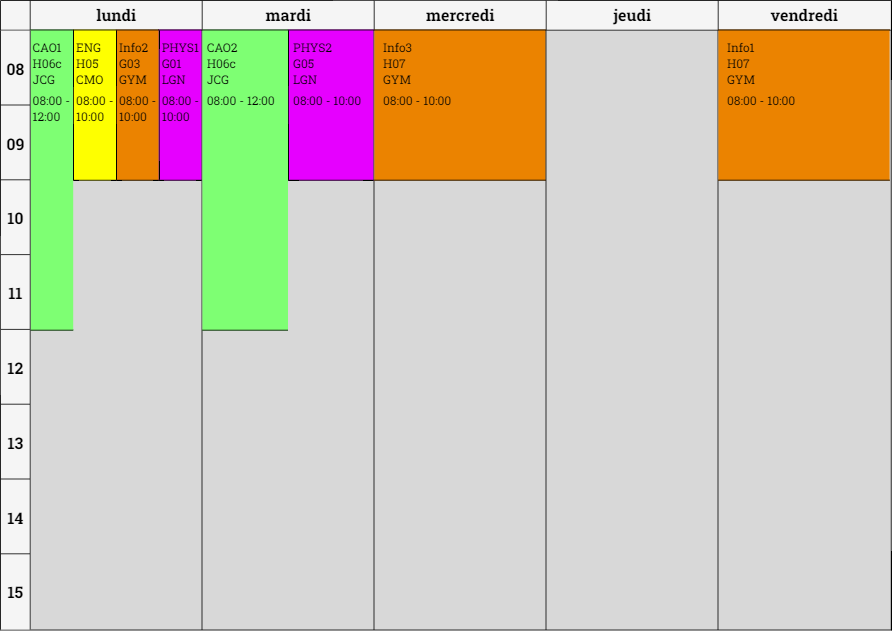
\includegraphics[width=1\textwidth]{./assets/figures/schedule.png}
\caption{Exemple d'horaire obtenu}
\end{figure}

\clearpage
\printbibliography

\appendix
\appendixpage
\addappheadtotoc

%%if
\chapter{Première annexe}

Les annexes n'ont pas un contenu \underline{normatif} mais \underline{descriptif}. Tout contenu annexé ne doit pas être nécessaire à la bonne compréhension du travail.

Les annexes contiennent généralement :

\begin{itemize}
    \item les dessins mécaniques (mises en plan);
    \item les schémas électriques détaillés;
    \item des photographies du projet;
    \item des scripts et des extraits de code source;
    \item des documents techniques \pex \emph{datasheet};
    \item des développements mathématiques.
\end{itemize}
\section{Sous section}
\lipsum[1]
%%fi

\let\cleardoublepage\clearpage
\backmatter

\label{glossaire}
\printnoidxglossary
\label{index}
\printindex

% Le colophon est le dernier élément d'un document qui contient des notes de l'auteur concernant la mise en page et l'édition du document : il est parfaitement optionnel.
%%if
\clearpage
\Large\textbf{Colophon :}\par\normalsize
\thispagestyle{empty}
La qualité de cet ouvrage repose que le moteur \LaTeX. La mise en page et le format sont inspirés d'ouvrages scientifiques tels que le modèle de thèse de l'EPFL et celui des publications O'Reilly.

Les diagrammes et les illustrations sont édités depuis l'outil en ligne draw.io. Certaines illustrations ont été reprises dans Adobe Illustrator. Les représentations 3D sont exportées de SolidWorks et certains graphiques sont générés à la volée depuis un code source Python.

L'auteur fictive de ce document \emph{Maria Bernasconi} est un nom emprunté, par amusement, aux spécimens publiés par Postfinance.

Ce document a été compilé avec XeLaTeX.

La famille de police de caractères utilisée est \emph{Computed Modern} créée par Donald Knuth avec son logiciel METAFONT.
\vfil
Le Colophon est le dernier élément d'un document qui contient des notes de l'auteur concernant la mise en page et l'édition du document : il est parfaitement optionnel.
%%fi

\end{document}
